% !TEX root = MAIN.tex

\chapter{Software Configuration Item Overview}

\section{Brief Description}

\begin{figure}[t]
  \centering
	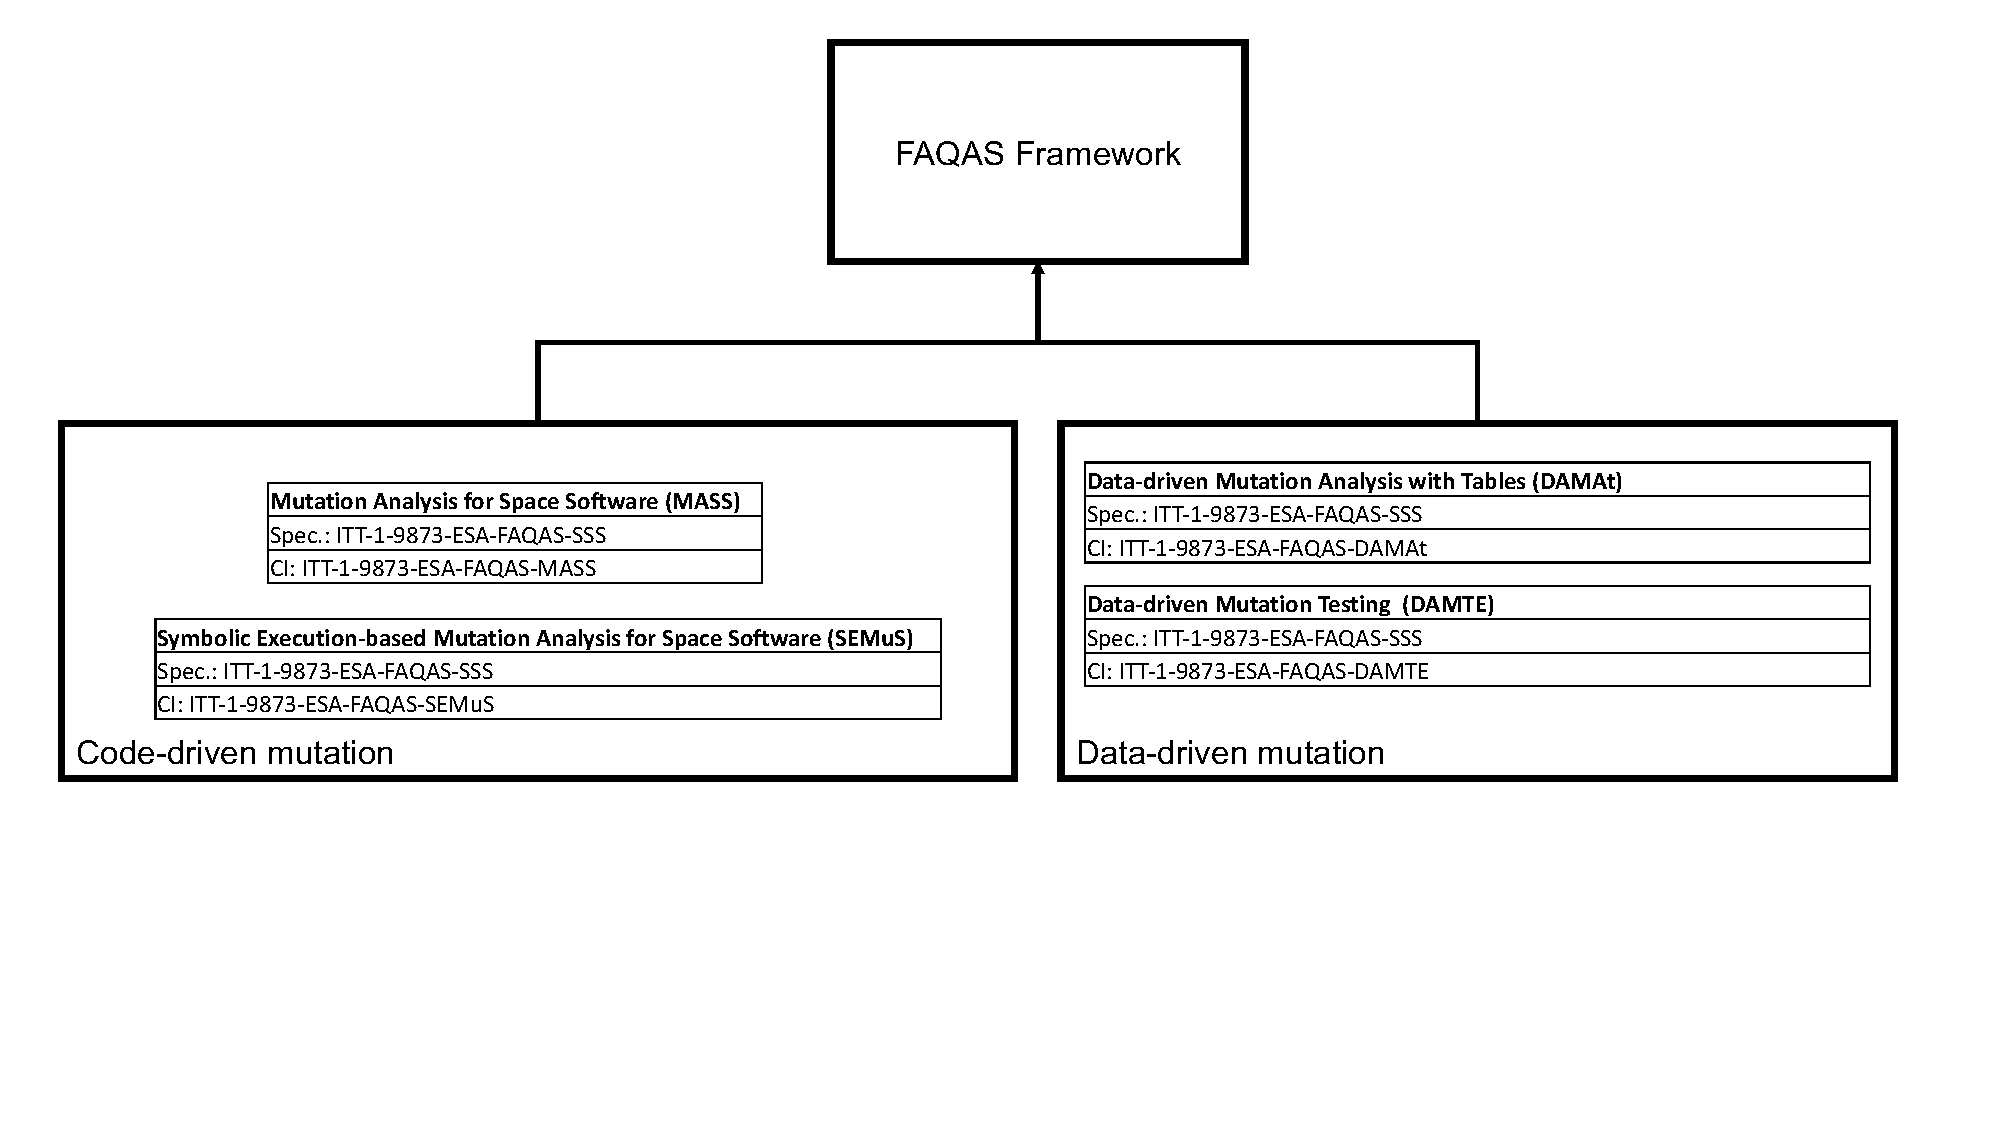
\includegraphics[width=\textwidth]{images/CI_tree.pdf}
      \caption{Product tree and identification of configuration items.}
      \label{fig:ci:tree}
\end{figure}


The software configuration item for the SCF consists of the software deliverables of FAQAS framework (i.e., \MASS, \SEMUS, \DAMA). The FAQAS framework is designed to be used for testing space software running in UNIX environments. The goal of the software include in this CI is to facilitate the verification and validation of ECSS compliant systems' test suites.

Figure~\ref{fig:ci:tree} shows all software configuration items within the FAQAS project. This document describes the software ITT-1-9873-ESA-FAQAS-MASS, ITT-1-9873-ESA-FAQAS-SEMuS, and ITT-1-9873-ESA-FAQAS-DAMAt.

\section{Information about the CI}

All information about the software contained in this configuration item (i.e., \MASS, \SEMUS, \DAMA) is stored in the documents specified in Chapter~\ref{chapter:baseline}; the procedure on how to build and use the different software can be found in the Software User Manual (SUM), and the Software Reuse File (SRF), defines the software reused in this project.

The platform to track the development process is the European Space Agency GitLab Repository\footnote{\url{https://gitrepos.estec.esa.int}}; the platform provides a Git repository where the development of each source code file can be traced. Precisely,
\STARTCHANGEDFINAL
\begin{itemize}
\item The issue tracker of the whole project is available at \url{https://gitlab.uni.lu/fpastore/FAQAS/}.
\item The repository of FAQAS is at \url{https://gitrepos.estec.esa.int/external/FAQAS}
\item The FAQAS tools can be found in the following sub-folders:
\begin{itemize}
    \item The MASS toolset is at \url{https://gitrepos.estec.esa.int/external/FAQAS/-/tree/master/MASS}
    \item The DAMAT toolset is at \url{https://gitrepos.estec.esa.int/external/FAQAS/-/tree/master/DAMAT}
    \item The SEMuS toolset is at \url{https://gitrepos.estec.esa.int/external/FAQAS/-/tree/master/SEMUS}
    \item The DAMTE toolset is at \url{https://gitrepos.estec.esa.int/external/FAQAS/-/tree/master/DAMTE}
\end{itemize}
\end{itemize}
\ENDCHANGEDFINAL

\section{CI Composition}

The CI documentation is provided in Chapter~\ref{chapter:baseline}, while the corresponding software source code and building procedures are listed in Section~\ref{sec:code_list}.

\section{Means to Develop, Modify, Install, and Run the CI}

The CI is delivered as source code. The instructions to install and execute the CI are described in the SUM document, while for the specifications and design of the software the Software Design Document (SDD), and Software System Specification (SSS) document shall be consulted.

